\documentclass[crop=false]{standalone}
\usepackage{standard}
\begin{document}
  \section{Einleitung} % (fold)
  \label{sec:introduction}

    In der Physik werden wichtige Vorgänge der Natur oder technischer Prozesse häufig durch partielle Differentialgleichungen beschrieben.
    Gerade in der industriellen Forschung und den Ingenieurswissenschaften benötigt man Lösungen dieser Gleichungen, um neue Bauteile und Verfahren, die gewissen Bedingungen genügen müssen, zu konstruieren.
    Als Beispiel sei hier die Wärmeleitungsgleichung genannt, deren Lösung es ermöglicht, die Temperaturverteilung und den Wärmetransport eines solchen Bauteils zu bestimmen.
    Die Lösungen weisen auf die Schwächen und Stärken des Bauteils hin, ohne dieses real konstruieren zu müssen.
    \cite{Schweizer2013,Logan2007}

    Die partiellen Differentialgleichungen zusammen mit der Geometrie der Bauteile und den Materialeigenschaften praxisnaher Probleme sind jedoch meistens zu kompliziert, um sie analytisch zu lösen.
    Entweder es existiert nicht einmal eine geschlossene Lösung oder sie wäre viel zu kompliziert.
    Aus diesem Grund beschränkt man sich in diesen Bereichen auf verschiedene numerische Verfahren, die die Gleichungen, die Geometrie und Materialeigenschaften diskretisieren und in ein System algebraischer Gleichungen transformieren.
    Die erhaltenen Ergebnisse des diskretisierten Systems stellen zwar nur eine Approximation der eigentlichen Lösung dar, können diese jedoch meistens beliebig genau annähern.
    Typische Verfahren zum Lösen von partiellen Differentialgleichungen stellen die Finite-Differenzen-Methode, die Finite-Volumen-Methode und die Finite-Elemente-Methode dar.
    In Abbildung \ref{fig:intro} wird die numerische Simulation der Wellengleichungen über mehrere Zeitschritte hinweg anhand eines Beispiels demonstriert, indem die Finite-Elemente-Methode verwendet wurde.
    \cite{Schweizer2013,Logan2007,Cheney2008,Quarteroni2000}

    \begin{figure}[h]
      \center
      \begin{subfigure}[b]{0.32\textwidth}
        \center
        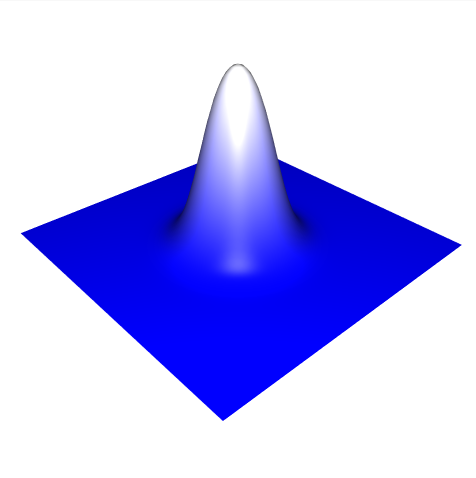
\includegraphics[trim={0 0 0 2.2cm}, clip, width=0.8\textwidth]{images/intro_01.png}
        \caption{}
      \end{subfigure}
      \begin{subfigure}[b]{0.32\textwidth}
        \center
        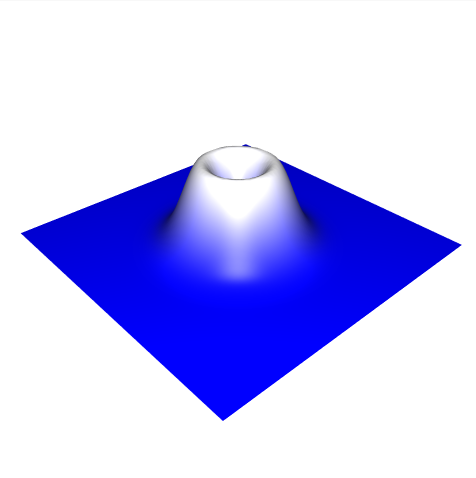
\includegraphics[trim={0 0 0 2.2cm}, clip, width=0.8\textwidth]{images/intro_02.png}
        \caption{}
      \end{subfigure}
      \begin{subfigure}[b]{0.32\textwidth}
        \center
        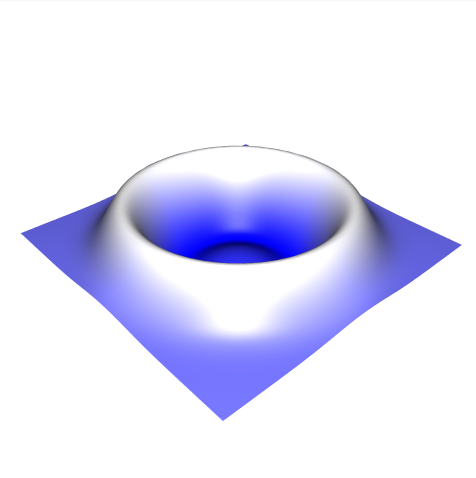
\includegraphics[trim={0 0 0 2.2cm}, clip, width=0.8\textwidth]{images/intro_03.png}
        \caption{}
      \end{subfigure}

      \begin{subfigure}[b]{0.32\textwidth}
        \center
        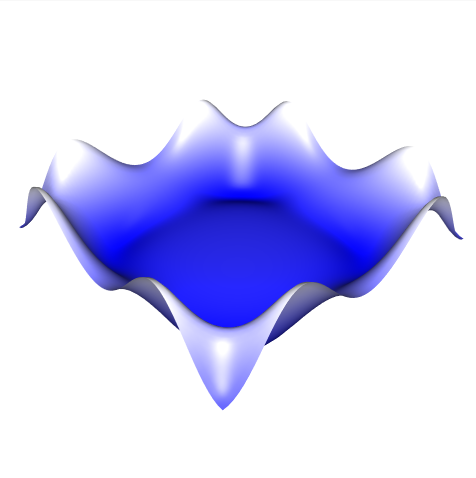
\includegraphics[trim={0 0 0 2.2cm}, clip, width=0.8\textwidth]{images/intro_04.png}
        \caption{}
      \end{subfigure}
      \begin{subfigure}[b]{0.32\textwidth}
        \center
        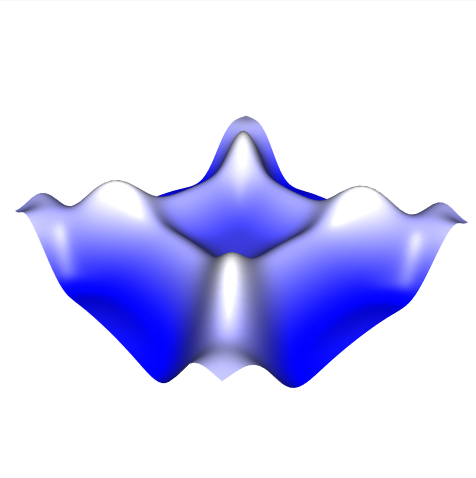
\includegraphics[trim={0 0 0 2.2cm}, clip, width=0.8\textwidth]{images/intro_05.png}
        \caption{}
      \end{subfigure}
      \begin{subfigure}[b]{0.32\textwidth}
        \center
        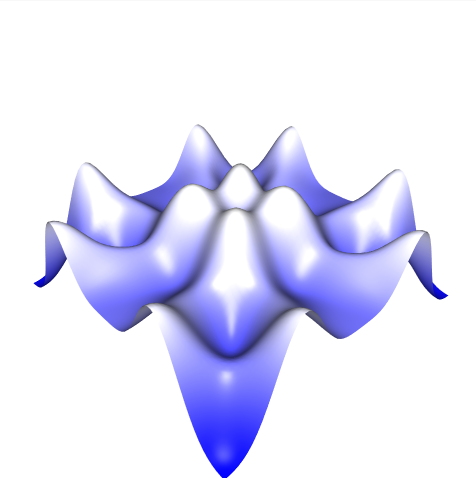
\includegraphics[trim={0 0 0 2.2cm}, clip, width=0.8\textwidth]{images/intro_06.png}
        \caption{}
      \end{subfigure}
      \caption[%
        Einfache Simulation der Wellengleichung%
      ]{%
        Die Abbildung zeigt die Evolution einer numerischen Lösung der Wellengleichung auf einem quadratischen zweidimensionalen Gebiet.
        Für die Berechnung wurde die hier implementierte Finite-Elemente-Methode verwendet.%
      }
      \label{fig:intro}
    \end{figure}

    Die Finite-Elemente-Methode stellt eines der allgemeinsten Verfahren zum numerischen Lösen von partiellen Differentialgleichungen dar.
    Einer ihrer größten Vorteile besteht darin, komplexe Geometrien und Randbedingungen durch die Art der Diskretisierung beliebig genau beschreiben zu können.
    Gerade deshalb tendiert die Finite-Elemente-Methode dazu, enorme Rechenleistungen zu benötigen, um die resultierenden algebraischen Gleichungen zu lösen.
    Allerdings konnte sie aufgrund ihrer im Vergleich zu anderen Verfahren späten Entwicklung durch ein mathematisches Vorgehen computergerecht formuliert werden, sodass Implementierungen dieser Methode die Hardware des Computers im Allgemeinen effizient ausnutzen.
    Demnach ist die Anwendung der Finite-Elemente-Methode nicht auf ein konkretes physikalisches Gebiet beschränkt.
    Obwohl sie zunächst nur für die Strukturberechnung von Flugzeugflügeln in der Luft- und Raumfahrtindustrie verwendet wurde, findet sie heute in vielen Bereichen der Physik, wie zum Beispiel bei der Berechnung des Wärmetransports, der Strömungssimulation, der Festigkeits- und Verformungsuntersuchung von Festkörpern, der gekoppelten Feldberechnung und bei Wettervorhersagen, ihre Anwendung.
    \cite{Logan2007,Cheney2008,Quarteroni2000}

    Das allgemeine Ziel besteht nun darin immer komplexer werdende Probleme zu lösen, indem man in das zugrundeliegende Modell neue physikalische Effekte mit einbezieht oder die Diskretisierung des Modells verfeinert, um die genannten Effekte besser aufzulösen.
    Folglich ist es erforderlich die Performance eines Programms immer weiter zu steigern.
    Dies erreicht man heutzutage durch dessen Parallelisierung.
    Aufgrund der computergerechten Formulierung der Finite-Elemente-Methode tritt bei ihr eine gewisse Datenparallelität auf.
    Bei dieser Tatsache handelt sich um eine Eigenschaft, die durch die Verwendung des Grafikprozessors (GPU) eines Computers ausgenutzt werden kann.
    Die GPU ist ein massiv-paralleler Prozessor, dessen Prozessorkerne auf die Ausnutzung von Datenparallelität innerhalb einer Gruppe von Threads spezialisiert sind.
    Ein Algorithmus der diese Parallelität nicht aufweist, lässt sich im Allgemeinen nur sehr ineffizient auf der GPU implementieren und sollte durch den Hauptprozessor (CPU) eines Computers, dessen Prozessorkerne für wesentlich komplexere Aufgaben designet wurden, ausgeführt werden.
    Umgekehrt ist die GPU in der Lage Algorithmen mit dieser Eigenschaft um ein Vielfaches zu beschleunigen.
    Gerade bei der Finite-Elemente-Methode sollte also die Implementierung auf der GPU diverse Vorteile mit sich bringen.
    \cite{Patterson2011,Kirk2010,Sanders2011}

  % section einführung (end)
\end{document}